\chapter{Graph Games}
This section gives an alternative definition of a combinatorial game.
This definition allows us to study general combinatorial games.
\begin{definition}
  A directed graph $G$ is a pair $(V, N)$ such that $F$ is a non-empty set and
  $F : V \to 2^V$.\footnote{We are going to have a more in-depth discussion
  of graphs in \Cref{part:graph-theory}.}

  We say that a game on $G$ is the game where elements of $V$ are positions
  and each player can move from $x \in V$ to any $y \in N(x)$. (Elements of
  $N(x)$ are called followers of $x$.)
\end{definition}

For example, the take-away game from \Cref{chapter:combinatorial-games}
can be considered as a graph on a graph $G = (\N_0, N)$,
where $N(0) = \emptyset$, $N(1) = \set{0}$, $N(2) = \set{0, 1}$, and
$N(n + 3) = \set{n, n + 1, n + 2}$ for any $n \in \N_0$.

The key ingreadient for the analisis of games based on graphs was proposed
by Sprague and Grundy. They proposed to consider the following function:
\begin{definition}
  Let $G = (V, N)$ be a directed graph. A function $g : V \to \N$ is a
  Sprague--Grundy function for $G$ iff
  $g(x) = \mex\set[y \in N(x)]{g(y)}$, where
  $\mex S = \min \set[n \notin S]{n \in \N_0}$.
\end{definition}


Consider the following graph (arrows depict possible moves).
\begin{center}
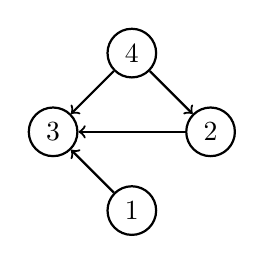
\begin{tikzpicture}[thick]
  \node[circle, draw, minimum size=6pt] (v1) at (0,0) {$1$};
  \node[circle, draw, minimum size=6pt] (v2) at (1,1) {$2$};
  \node[circle, draw, minimum size=6pt] (v3) at (-1,1) {$3$};
  \node[circle, draw, minimum size=6pt] (v4) at (0,2) {$4$};


  \draw[->] (v2) -- (v3);
  \draw[->] (v1) -- (v3);
  \draw[->] (v4) -- (v3);
  \draw[->] (v4) -- (v2);
\end{tikzpicture}
\end{center}
Let us assume that $g$ is a Sprague--Grundy funciton for this graph.
Note that $3$ is a terminal position so $g(3) = \mex \emptyset = 0$.
Since from $1$ and $2$ there are only moves to $3$, it is clear that
$g(1) = g(2) = \mex \set{0} = 1$. Finally, $g(4) = \mex \set{0, 1} = 2$.

Note that the Sprague--Grundy function is recursively defined so it may
not exist or not to be unique if graph has cycles; i.e. if there are $x_1,
\dots, x_n$ such that $x_2 \in N(x_1)$, \dots, $x_n \in N(x_{n - 1})$, and 
$x_1 \in N(x_1)$.
For example, the graph depicted on \Cref{figure:sprague-grundy-not-exists}
does not have a Sprague--Grundy function.
Indeed, assume that such a function $g$ exists. Consider two following cases.
\begin{itemize}
    \item Firs case is when $g(3) = 0$. Note that $g(2) = \mex \set{0} = 1$.
        Hence, $g(1) = \mex \set{1} = 0$ which contradicts to the assumption
        that $g(3) = 0$ since $g(3) = \mex \set{g(0)} = 1$.
    \item Firs case is when $g(3) \neq 0$. Note that $g(2) = \mex \set{g(3)} = 0$.
        Therefore $g(1) = \mex \set{0} = 1$ and $g(3) = \mex \set{1} = 0$ which
        is a contradiction.
\end{itemize}

Note that the graph depicted on \Cref{figure:sprague-grundy-not-unique} has
several Sprague--Grundy functions. We may consider functions $g_1$ and $g_2$
such that $g_1(1) = g_1(3) = g_2(2) = g_2(4) = 0$ and
$g_2(1) = g_2(3) = g_1(2) = g_1(4) = 1$. It is clear that they are
Sprague--Grundy functions for the graph from
\Cref{figure:sprague-grundy-not-unique}.

\begin{figure}
    \centering
    \subfloat[A graph without a Sprague--Grundy function
              \label{figure:sprague-grundy-not-exists}]{
      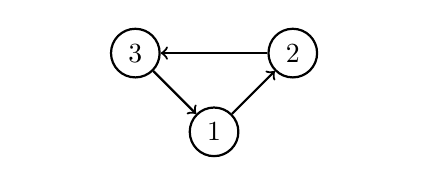
\begin{tikzpicture}[thick]
        \node[circle, draw, minimum size=6pt] (v1) at (0,0) {$1$};
        \node[circle, draw, minimum size=6pt] (v2) at (1,1) {$2$};
        \node[circle, draw, minimum size=6pt] (v3) at (-1,1) {$3$};
        \node[] (dummy) at (2.25,1) {};
        \node[] (dummy) at (-2.25,1) {};

        \draw[->] (v1) -- (v2);
        \draw[->] (v2) -- (v3);
        \draw[->] (v3) -- (v1);
      \end{tikzpicture}
    }
    \qquad
    \subfloat[A graph with several Sprague--Grundy functions
              \label{figure:sprague-grundy-not-unique}] {
      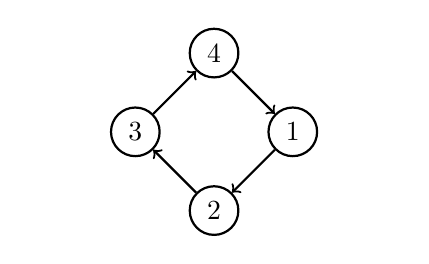
\begin{tikzpicture}[thick]
        \node[circle, draw, minimum size=6pt] (v1) at (1,1) {$1$};
        \node[circle, draw, minimum size=6pt] (v2) at (0,0) {$2$};
        \node[circle, draw, minimum size=6pt] (v3) at (-1,1) {$3$};
        \node[circle, draw, minimum size=6pt] (v4) at (0,2) {$4$};
        \node[] (dummy) at (2.25,1) {};
        \node[] (dummy) at (-2.25,1) {};


        \draw[->] (v1) -- (v2);
        \draw[->] (v2) -- (v3);
        \draw[->] (v3) -- (v4);
        \draw[->] (v4) -- (v1);
      \end{tikzpicture}
    }
    \caption{Graphs where Sprague--Grundy function is either not unique or does
      not exist.}
    \vskip 10pt
\end{figure}

Unfortunately, even if there are no cycles, a graph my not have a
Sprague--Grundy function or have several Sprague--Grundy functions. Indeed,
consider the graph $G = (\Z, N)$ such that $N(x) = \set{x - 1}$. It is clear
that the functions $g_1$ and $g_2$ such that
\begin{gather*}
    g_1(x) =
    \begin{cases}
        0 & \text{if } x \text{ is even} \\
        1 & \text{if } x \text{ is odd}
    \end{cases} \\
    \text{and} \\
    g_2(x) =
    \begin{cases}
        0 & \text{if } x \text{ is even} \\
        1 & \text{if } x \text{ is odd}
    \end{cases}
\end{gather*}
are Sprague--Grundy functions for $G$.

\begin{exercise}
    Let $G = (\N \cup \set{-1}, N)$ such that $F(x) = \set{x - 1}$ for $x \ge 1$,
    $N(0) = \emptyset$, and $N(-1) = \N$.
    Show that $G$ does not have a Sprague--Grundy function.
\end{exercise}

However, for almost all the combinatorial games we are going to consider
the Sprague--Grundy function exists and is unique.
Let $g$ be a Sprague--Grundy funciton for \Cref{game:take-away-21-3-2-1}.
We are going to show that it is unique.
Note that if $x$ is a terminal position, then $g(x) = 0$. Hence, $g(0) = 0$.
There is only one move from $1$ so $g(1) = \mex \set{0} = 1$. Similarly
there are two moves from $2$: one to $1$ and one to $0$ so
$g(2) = \mex \set{0, 1} = 2$. In the same way $g(3) = \mex \set{0, 1, 2} = 3$
and $g(4) = \mex \set{1, 2, 3} = 0$.
One may notice that there is a pattern and conjecture that
\[
  g(x) =
  \begin{cases}
      0 & \text{if } x \equiv 0 \pmod{4} \\
      1 & \text{if } x \equiv 1 \pmod{4} \\
      2 & \text{if } x \equiv 2 \pmod{4} \\
      3 & \text{if } x \equiv 3 \pmod{4}
  \end{cases}.
\]
We already proved the base case, let us now prove the induction step.
Assume the equality is true for all $y < x$ and consider the following cases.
\begin{itemize}
    \item If $x \equiv 0 \pmod{4}$, then $x - 1 \equiv 3 \pmod{4}$,
        $x - 2 \equiv 2 \pmod{4}$, and $x - 3 \equiv 1 \pmod{4}$.
        Hence, $g(x) = \mex \set{1, 2, 3} = 0$.
    \item If $x \equiv 1 \pmod{4}$, similarly $g(x) = \mex \set{2, 3, 0} = 1$.
    \item If $x \equiv 2 \pmod{4}$, $g(x) = \mex \set{3, 0, 1} = 2$.
    \item If $x \equiv 3 \pmod{4}$, $g(x) = \mex \set{0, 1, 2} = 3$.
\end{itemize}
It is also clear that the constructed function is indeed a Sprague--Grundy
function for \Cref{game:take-away-21-3-2-1}. Therefore we proved that
existence and uniqueness.
\begin{table}
  \centering
  \begin{tabular}{l l l l l l l l l}
      \toprule
      0 & 1 & 2 & 3 & 4 & 5 & 6 & 7 & 8 \\
      \midrule
      0 & 1 & 2 & 3 & 0 & 1 & 2 & 3 & 0 \\
      \bottomrule
  \end{tabular}
  \caption{The Sprague--Grundy funciton for \Cref{game:take-away-21-3-2-1}}
  \label{table:take-away-21-3-2-1-grundy}
\end{table}

Note that P-positions are the positions where $g$ is zero. In fact,
this is not a coincidence.
\begin{theorem}
\label{theorem:grundy-to-np}
    Let $G$ be a graph such that there is a unique Sprague-Grundy function for
    $G$. Then a position $x$ in the game on $G$ is a P-position iff $g(x) = 0$.
\end{theorem}


\begin{chapterendexercises}
    \exercise Prove \Cref{theorem:grundy-to-np}.
    \exercise Show that there are only two Sprague--Grundy functions for the
    graph depicted on \Cref{figure:sprague-grundy-not-unique}.
    \exercise Prove that there is unique Sprague--Grundy function for the one pile
        Nim game.
    \exercise Prove that there is unique Sprague--Grundy function for the
        subtraction game where players may subtract $2$ and $3$ chips on their
        turn.
    \exercise
       Prove that there is unique Sprague--Grundy function for the subtraction
       game where players may subtract $1$, $2$, or $5$ chips
       on their turn.
\end{chapterendexercises}
